\chapter{The Library}

\section{General Idea}
% explain how it works
A brief description of how \gnutls{} works internally is shown at
the figure \ref{fig:internals}.

\begin{figure}[htp]
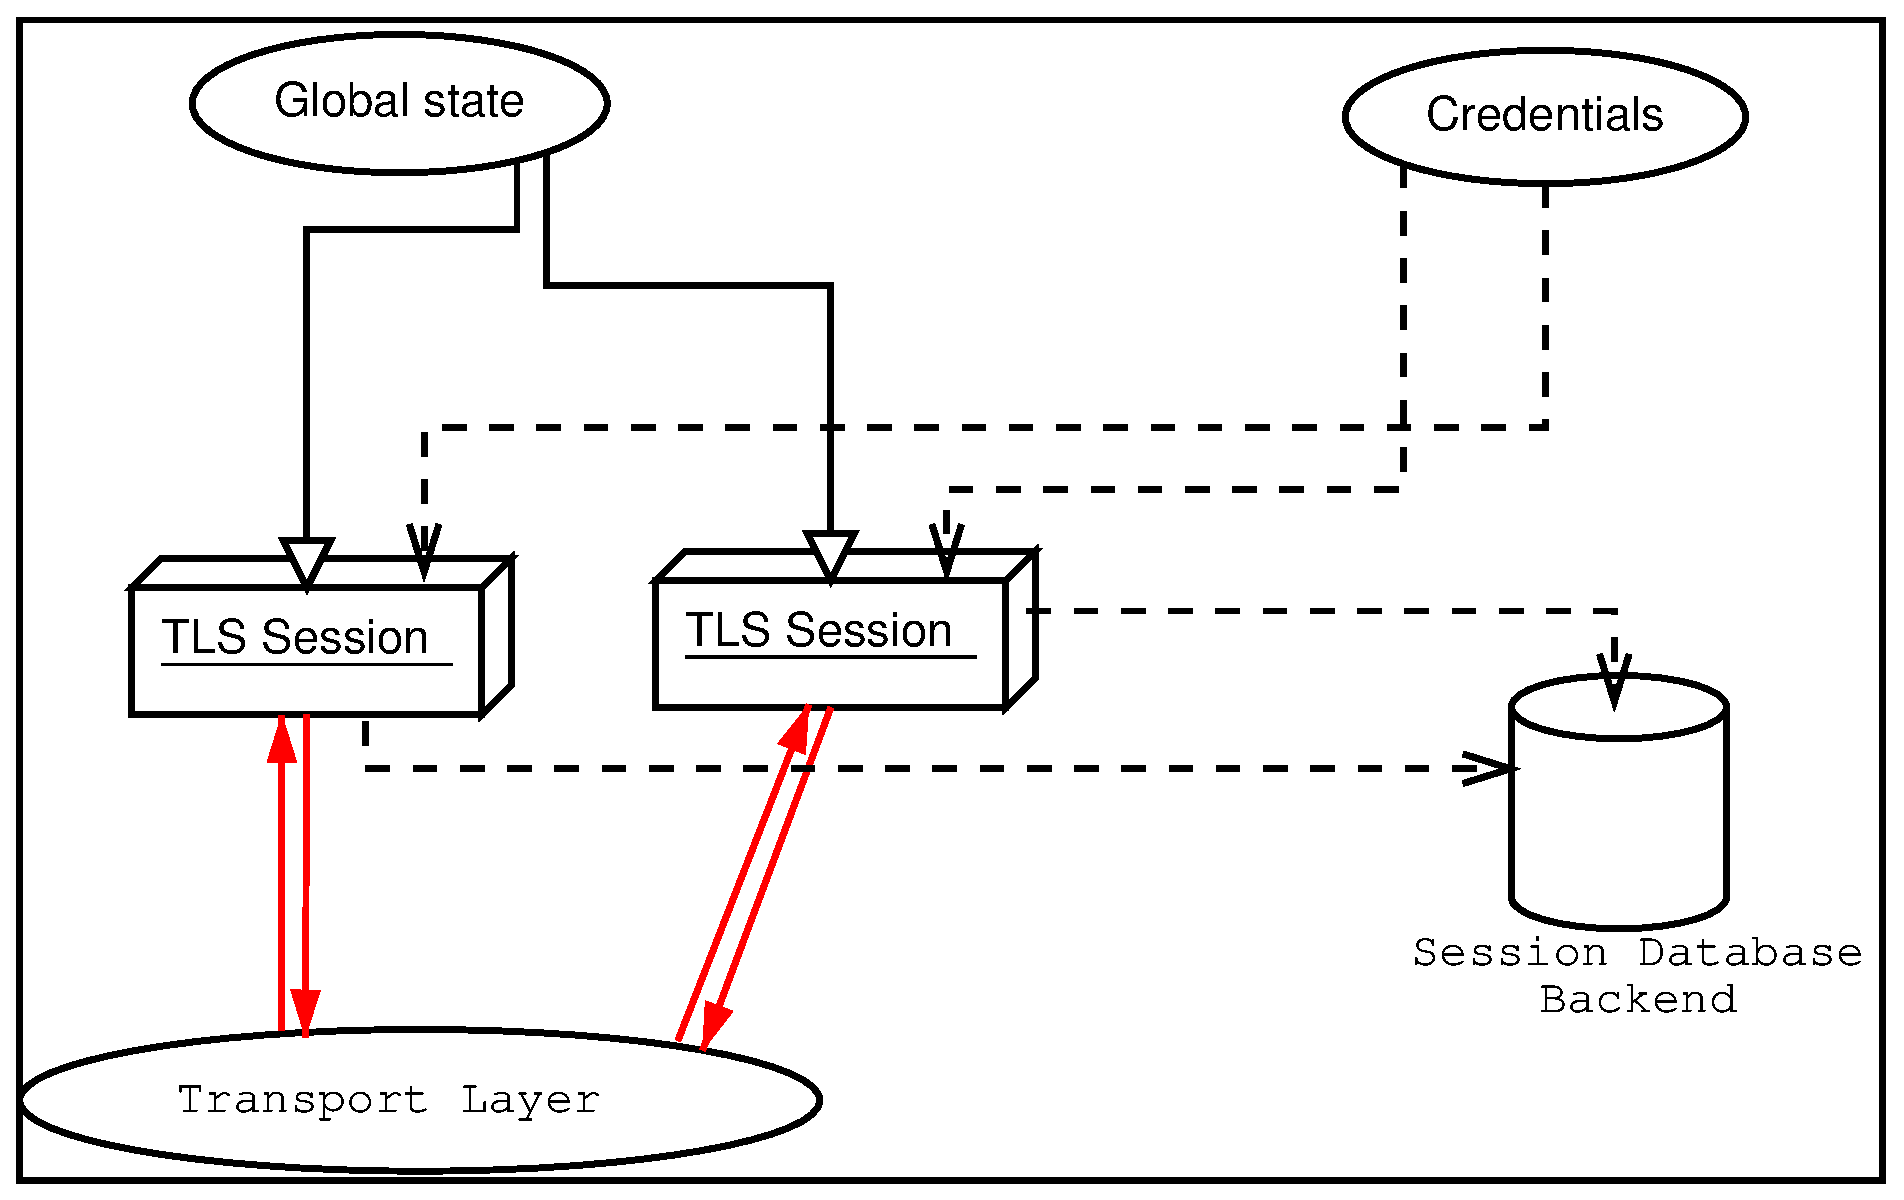
\includegraphics[height=8cm,width=12cm]{internals}
\label{fig:internals}
\end{figure}

\section{Error Handling}
\par
In \gnutls most functions return an integer type as a result.
In almost all cases a zero or a positive number means success, and
a negative number indicates failure, or a situation that some
action has to be taken. Thus negative error codes may be fatal
or not. 
\par 
Fatal errors terminate the connection immediately and
further sends ard receives will be disallowed. An example of
a fatal error code is GNUTLS\_E\_MAC\_FAILED. Non-fatal errors
may warn about something (ie a warning alert was received), or
indicate the some action has to be taken. This is the case with
the error code GNUTLS\_E\_REHANDSHAKE returned by 
\hyperref{gnutls\_record\_recv()}{gnutls\_record\_recv() (see Section }{)}{gnutls_record_recv}.
This error code indicates that the server requests a rehandshake. The client
may ignore this request, or may reply with an alert.
You can test if an error code is a fatal one by using the
\hyperref{gnutls\_error\_is\_fatal()}{gnutls\_error\_is\_fatal() (see Section }{)}{gnutls_error_is_fatal}.
\par
If any non fatal errors, that require reaction, are to be returned by a
function, these error codes will be documented
in the function's reference.



\section{Memory handling}

\gnutls{} internally handles heap allocated objects differently, depending
on the sensitivity of the data they contain. However for performance
reasons, the default memory functions do not overwrite sensitive data from
memory, nor protect such objects from being written to the swap. 
In order to change the default behavior the
\printfunc{gnutls_global_set_mem_functions}{gnutls\_global\_set\_mem\_functions}
function is available which can be used to set other memory 
handlers than the defaults. 
\par
The \emph{libgcrypt} library on which \gnutls{} depends, has such secure
memory allocation functions available. These should be used in cases
where even the system's swap memory is not considered secure. See
the documentation of \emph{libgcrypt} for more information.



